\section{Methodology}
The methodology to achieve the objectives and outcomes for this project were divided into the 18 steps listed in table  \ref{method-objectives}.
\section{Design Specifications}
Prototypes 1 and 2 were designed with the following specifications. 

\subsection{System Design}

\begin{figure}[h]
	\centering
	\caption{Prototype 1 System Diagram}
	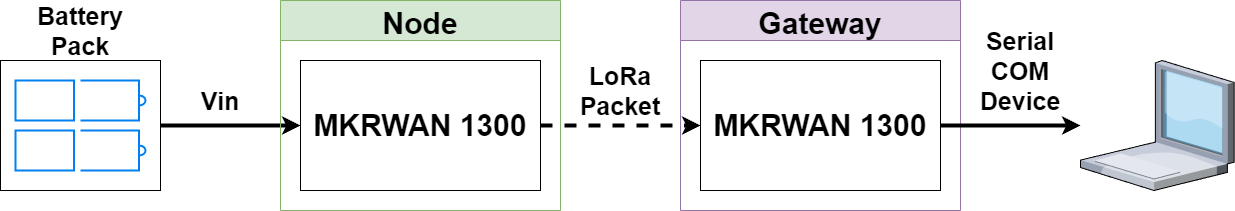
\includegraphics[width=\textwidth]{Sections/Design-Process/proto1-sys-diagram.png}
	\label{proto1-sys-diagram}
\end{figure}

The system diagram in figure \ref{proto1-sys-diagram} was used for initial testing in the beam experiment and has two variations. In the first variation the node is connected via COM device to a laptop and establishes serial connection. In the second variation there is no physical connection between the node and laptop and the node is powered via battery. The initial design with serial connection is so that the raw acceleration can be recorded since this is too much data to send over a LoRa packet. In both variations the node sends the maximum acceleration and peak frequency via LoRa packet to the gateway node. 

The system diagram in figure \ref{proto2-sys-diagram} forms the system design of prototype 2 and was used in the integrated testing and data collection on the Griffith footbridge. Since the gateway was unable to connect to the Griffith Wi-Fi due to security infrastructure, an Apple MacBook Pro was turned into a router using the inbuilt internet sharing option. A mobile phone hotspot was used to connect the laptop to the internet, and this was shared with the gateway via an Ethernet port. The gateway was configured in Basics Station mode, with TLS certificate and token authentication, and was connected to the Arduino IoT Cloud via the TNN Stack V3 back end integration via the LoRaWAN Network Server (LNS) sub protocol. The LoRa packets and message payloads are managed by TNN and are stored in Arduino Cloud variables. The Arduino Cloud Maker subscription offers 3 months of data retention which was used to plot the acceleration and frequency variables on two advanced graphs in the Arduino Cloud dashboard. This dashboard can be accessed on the laptop via the Arduino Cloud dashboard web page, or on the mobile phone via the Arduino IoT Remote app. Due to the cloud variable data retention, the variable history log can be downloaded in CSV format and plotted in excel. 

\begin{figure}[H]
	\centering
	\caption{Prototype 2 System Diagram}
	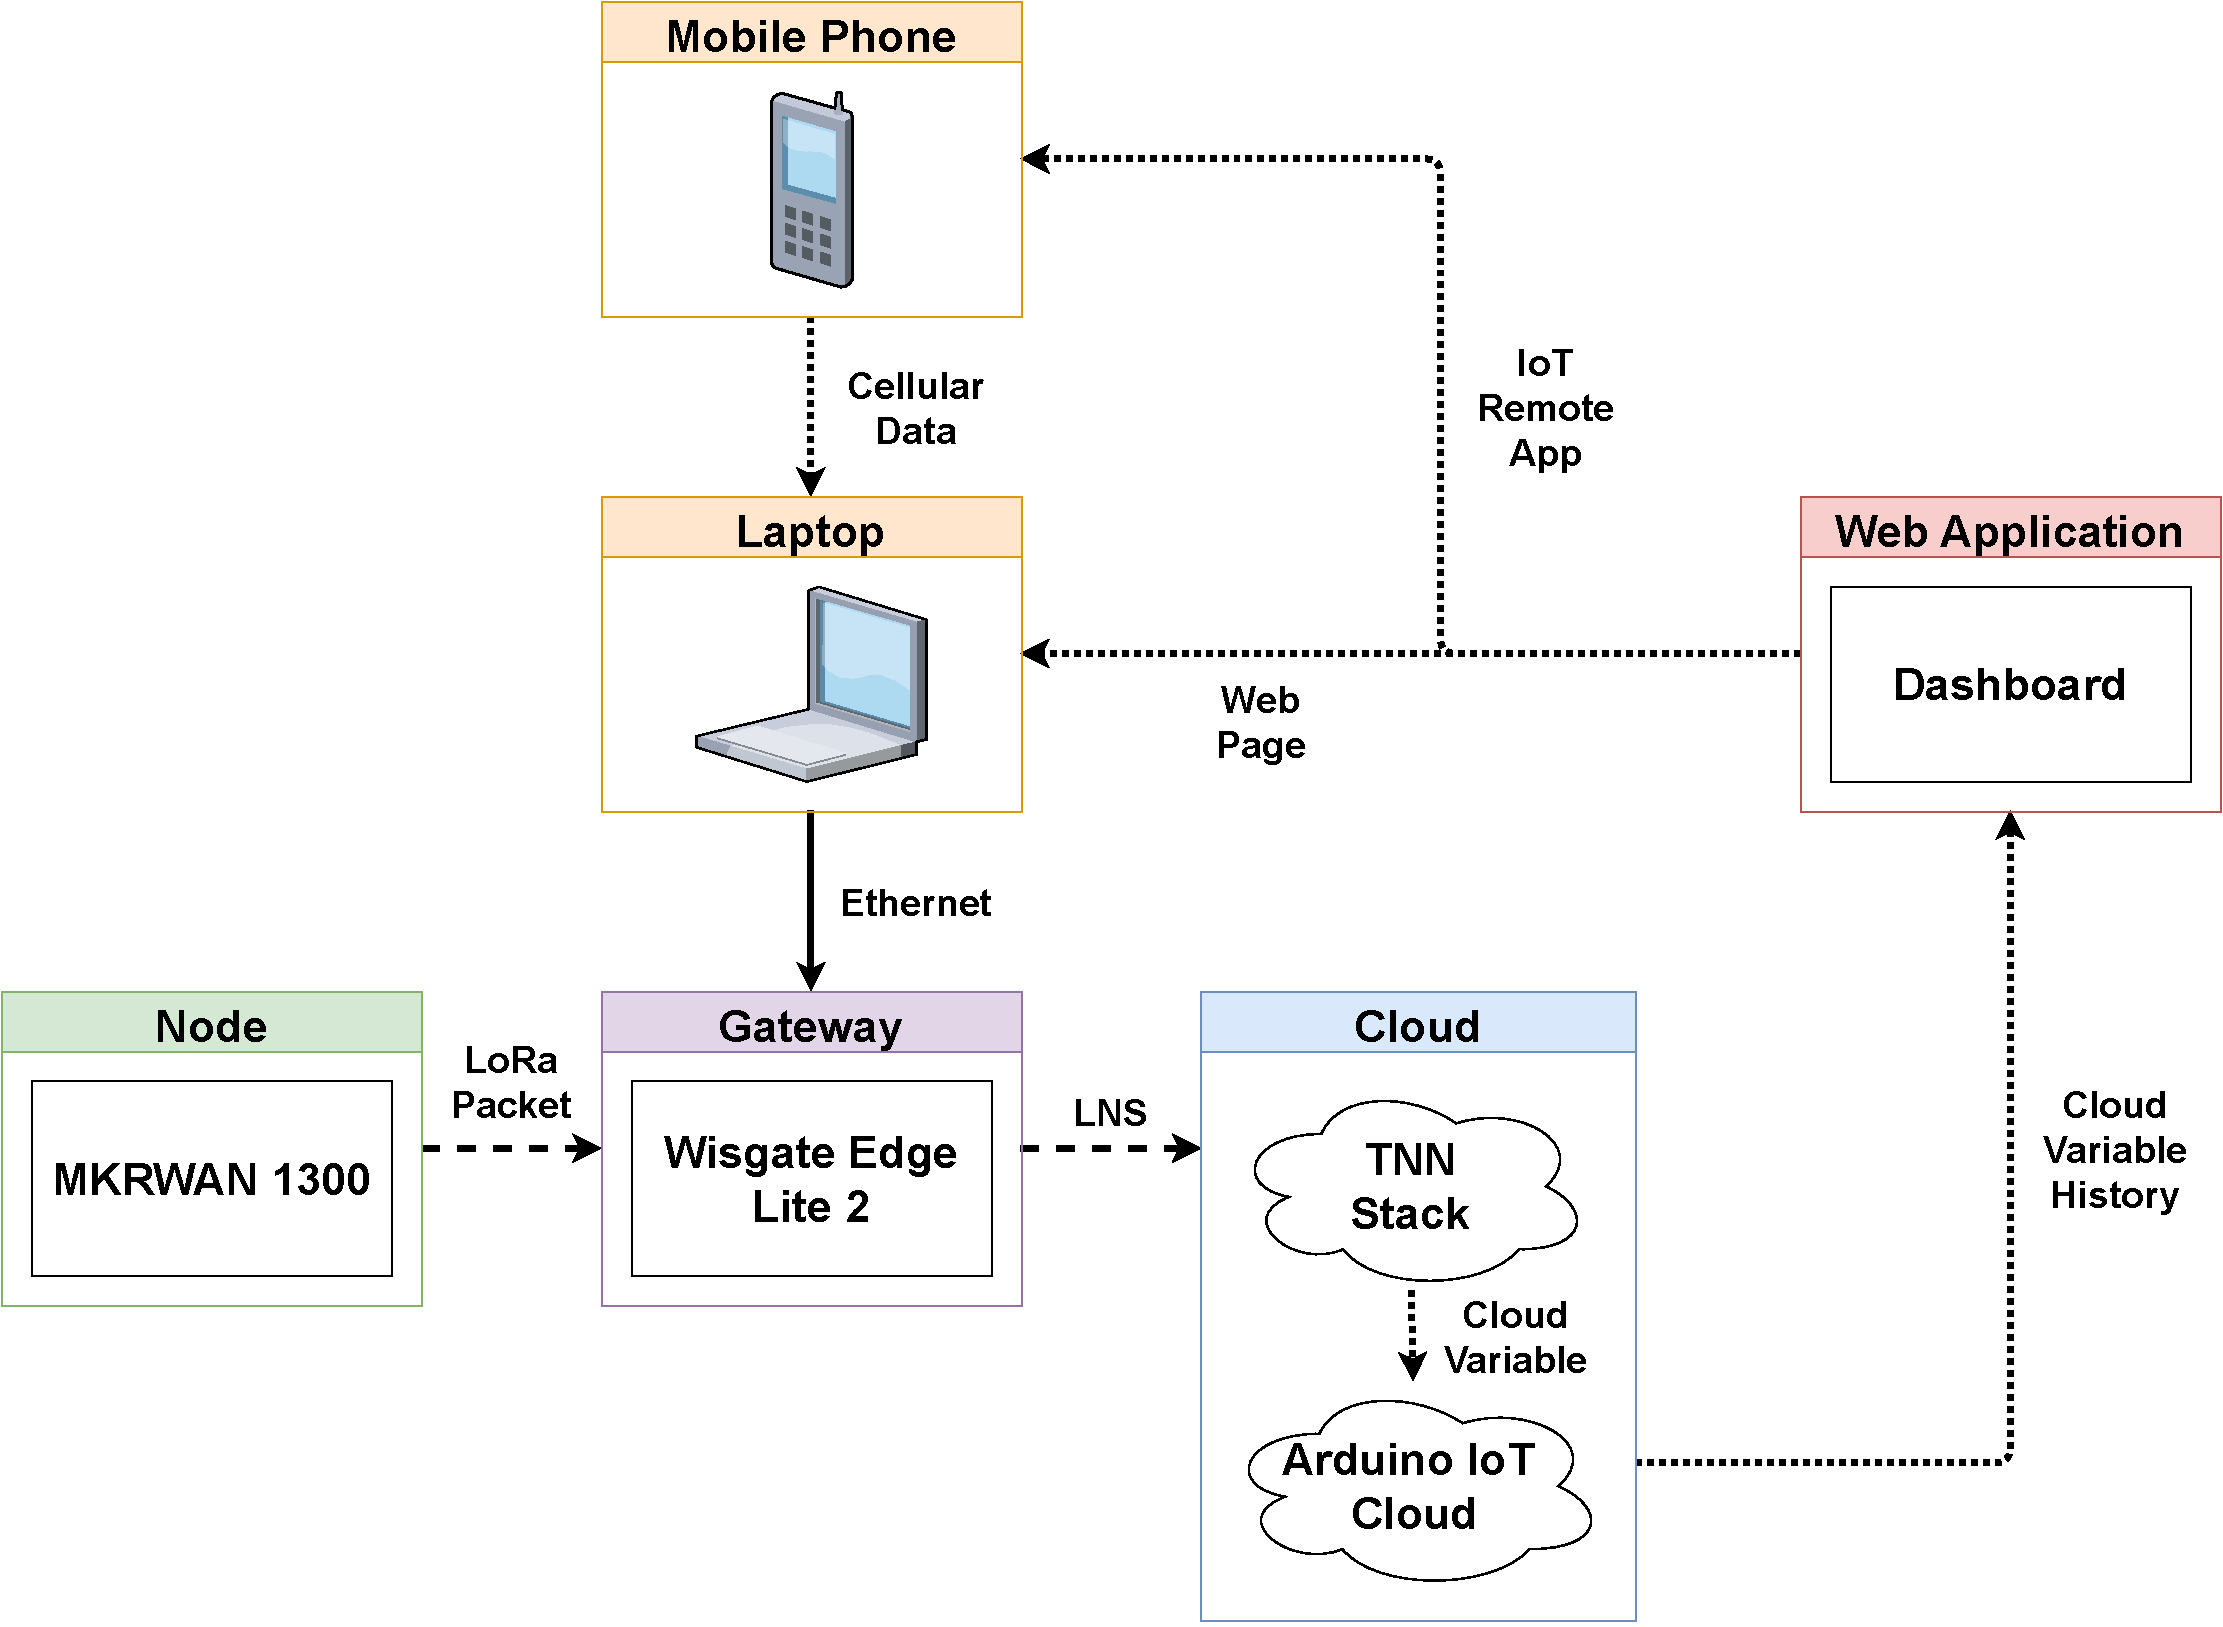
\includegraphics[width=\textwidth]{Sections/Design-Process/proto2-sys-diagram.pdf}
	\label{proto2-sys-diagram}
\end{figure}

\subsection{Data Processing}
\subsubsection{Sampling}
For the beam testing the sampling number (N) was 128, and for the bridge testing N increased to 256. A cut-off frequency ($F_c$) of 25 Hz was chosen, and according to the Nyquist theorem, the sampling Frequency (Fs) was chosen to be 50 Hz which meets the minimum value of $2 * F_c$ to avoid aliasing. This cut-off and sampling frequency are well above the desired 2 Hz to 3 Hz values and allow for higher frequencies to be shown, allowing for adjustments to the software. The sampling interval is then $\frac{1}{F_s}$, and substituting Fs with 50 Hz gives 0.02 seconds between each sample. This gives a total of 2.56 seconds to sample 128 values and 5.12 seconds to sample 256 values. 

\begin{table}[H]
\begin{tabular}{|c|l|}
\hline
\textbf{Step} & \multicolumn{1}{c|}{\textbf{Process}}                                                                                                                                                                                                                 \\ \hline
\textbf{1}    & \begin{tabular}[c]{@{}l@{}}Perform literature review on LoRaWAN technology. Determine\\ suitable steps to implement the IoT architecture.\end{tabular}                                                                                                \\ \hline
\textbf{2}    & \begin{tabular}[c]{@{}l@{}}Perform literature review on structural health monitoring and \\ existing WSN structural implementations.\end{tabular}                                                                                                     \\ \hline
\textbf{3}    & \begin{tabular}[c]{@{}l@{}}Examine results from FE analysis for beam experiment and \\ review the Griffith footbridge design paper to collect expected\\ first mode flexural frequencies.\end{tabular}                                                \\ \hline
\textbf{4}    & \begin{tabular}[c]{@{}l@{}}Determine the correct sampling parameters for the accelerometer\\ and choose a suitable FFT library.\end{tabular}                                                                                                          \\ \hline
\textbf{5}    & \begin{tabular}[c]{@{}l@{}}Implement the FFT library functions and test with a 2Hz sine \\ wave.\end{tabular}                                                                                                                                         \\ \hline
\textbf{6}    & \begin{tabular}[c]{@{}l@{}}Integrate the accelerometer data with the FFT functions and \\ determine the maximum acceleration and maximum frequency. \\ Implement a suitable low pass filter and noise thresholds for \\ data collection.\end{tabular} \\ \hline
\textbf{7}    & \begin{tabular}[c]{@{}l@{}}Develop software for the beam test experiment. This includes \\ Python code to log and plot serial data.\end{tabular}                                                                                                      \\ \hline
\textbf{8}    & \begin{tabular}[c]{@{}l@{}}Conduct beam experiment and review the plotted data. Adjust \\ filter and noise threshold values accordingly.\end{tabular}                                                                                                 \\ \hline
\textbf{9}    & Conduct node to node range test.                                                                                                                                                                                                                      \\ \hline
\textbf{10}   & Design PCB carrier board for microcontroller and accelerometer.                                                                                                                                                                                       \\ \hline
\textbf{11}   & Design and print enclosure for PCB and battery pack.                                                                                                                                                                                                  \\ \hline
\textbf{12}   & \begin{tabular}[c]{@{}l@{}}Solder connections from microcontroller, accelerometer and\\ battery pack to PCB.\end{tabular}                                                                                                                             \\ \hline
\textbf{13}   & \begin{tabular}[c]{@{}l@{}}Choose suitable LoRaWAN gateway and set up as basics station \\ mode. Add TLS authentication certificate and token to connect \\ to TNN.\end{tabular}                                                                      \\ \hline
\textbf{14}   & \begin{tabular}[c]{@{}l@{}}Register things and cloud variables in Arduino IoT cloud. Add \\ graphs in dashboard for cloud variables.\end{tabular}                                                                                                     \\ \hline
\textbf{15}   & \begin{tabular}[c]{@{}l@{}}Adapt code to store variables of interest in cloud variables and\\ sync with Arduino Cloud.\end{tabular}                                                                                                                   \\ \hline
\textbf{16}   & \begin{tabular}[c]{@{}l@{}}Install enclosure behind hand rail of Griffith footbridge. Setup \\ gateway and laptop nearby.\end{tabular}                                                                                                                \\ \hline
\textbf{17}   & \begin{tabular}[c]{@{}l@{}}Conduct bridge testing. Record the packet payload, SNR, RSSI\\ and spreading factor.\end{tabular}                                                                                                                          \\ \hline
\textbf{18}   & Determine the best noise thresholds through iterative testing.                                                                                                                                                                                        \\ \hline
\end{tabular}
\caption{Methodology to Achieve Project Objectives}
\label{method-objectives}
\end{table}



\subsubsection{Discretising the Accelerometer Readings}
The accelerometer values are input to the program via the Arduino analogRead() function. These raw values are represented as voltage changes ranging from 0-3V. In this scenario, 1.5 V represents the stationary state, 0V maximum acceleration in the negative direction and 3.0 V the maximum acceleration in the positive direction. The x, y and z axis are inputs to three of the MKRWAN1300's analog inputs, A1, A2 and A3. The microcontroller uses the on-board 12-bit analog to digital converter (ADC) to map these voltage readings to a corresponding discrete value between 0 and 4095. The acceleration is then calculated using the accelerometer's reference voltage which is 3.3 V when powered via USB and 3.0 V when powered via battery, and the accelerometer's sensitivity value which is 0.33 mV/g. The zero value is found during the calibration process of the accelerometer which will be outlined in the software design section. These values are multiplied by Earth's gravitational constant g (9.81 m/s/s) to convert the acceleration from G's to m/s/s. This process can be seen in equation \ref{ADC}. 1.0 m/s/s is subtracted from the z-axis for scenarios in which the z-axis is facing upwards to remove Earth's downwards directional gravity from this reading. A noise threshold is then applied to the acceleration values depending on the implementation to remove electrical noise from the signal. Equation \ref{ADC} is an example of generating processed acceleration values. 

\begin{equation} \label{ADC}
a[i] = \frac{\frac{a\_raw[i] * vRef}{adc\_resolution - 1} - \frac{vRef}{2}} {sensitivity - aZero} * g
\end{equation}

\subsubsection{Filtering}
A low-pass filter was applied to the processed acceleration values to remove high frequencies. The cut-off value for this filter was 5 Hz ($LP\_F_c$) and a smoothing factor of 0.283 was picked after experimental testing. The smoothing factor effectively acts as a weighting for the filter where higher values allow higher frequencies to pass through and lower values filter out high-frequency components. This filter effectively removes noise that was missed by the noise thresholds in the processed acceleration and ensures that no high frequencies due to small and rapid acceleration pass through. The smoothing factor for the low-pass filter was calculated with equation \ref{smoothing-factor}. 

\begin{equation} \label{smoothing-factor}
Smoothing\_Factor = \frac{1}{1 + (2 * \pi * LP\_F_c * (\frac{1}{F_s}))}
\end{equation}

\subsubsection{Fast Fourier Transform}
To facilitate the desired maximum frequency response of acceleration over time for both prototypes, the Arduino Fast Fourier Transform (FFT) library was used to convert the processed acceleration values into the respective frequency response. This frequency response was compared to the Strand7 Finite Elements (FE) simulation of the beam experiment and the Griffith footbridge documentation to validate the first mode flexural frequency (natural vertical frequency) for each of the prototypes. The predicted response of the FFT from the beam experiment is a steady peak of approximately 2.4 Hz, and the documented natural frequency of the bridge was 2.2 Hz.\\\\
When performing the FFT, N must be chosen as a power of two as defined in the library code. This is because the FFT is the most efficient when the sample window is to the power of two and so this condition is hard-coded into the library function, hence the values of N, 128 and 256 were chosen. The Hanning window was chosen for the FFT since it offers an adequate balance of frequency resolution and suitable distinction of frequency peaks. This window also minimizes spectral leakage which is helpful to distinguish between the frequency peaks due to acceleration and frequency peaks due to noise in the accelerometer. The FFT function assumed no imaginary values and used a complex to magnitude function to convert from polar to rectangular notation. 

\subsection{Design Resources}
The prototypes developed in this project required numerous programming tools, languages, electronics and materials. The microcontroller code was written in the C++ language in the Arduino IDE and the Python language was used for the logging and plotting scripts for prototype one. Altium Designer was used to design the PCB, and OnShape was used for the 3D modelling of the enclosure for prototype 2. The bill of materials for each prototype are displayed in table \ref{proto1-bom} and table \ref{proto2-bom}. This bill of materials does not include shipping costs. 

\subsection{Software Design}
The software design for this project is outlined in the software diagrams in figures \ref{proto1-soft-diagram}, \ref{proto1-soft-diagram-receiver}, \ref{proto1-soft-diagram-log}, \ref{proto1-soft-diagram-sender-plot}, \ref{proto1-soft-diagram-receiver-plot} and \ref{proto2-soft-diagram}. The software processing steps for each prototype are outlined in tables \ref{proto1-beam-test-soft-steps} and \ref{proto2-bridge-test-soft-steps}. 

\subsubsection{Import Libraries and Modules}
The external libraries and modules specified in steps 1, 10, 14 and 20 of table \ref{proto1-beam-test-soft-steps} and step 1 of table \ref{proto2-bridge-test-soft-steps} are listed in table \ref{module-list}. 

\subsubsection{Program Parameters}
The program parameters specified in steps 1, 10, 14 and 20 of table \ref{proto1-beam-test-soft-steps} and step 1 of table \ref{proto2-bridge-test-soft-steps} are listed in table \ref{global-vars}.

\subsubsection{Initializing LoRa and Serial Connection}
In the prototype 1 setup function for the sender and receiver programs, the serial connection is established with 9600 baud using the Serial.begin() function. This allows the microcontroller to print data serially to the Arduino IDE serial output. This also allows data to be logged via the serial connection within the logging and plotting Python scripts. Since the prototype one beam test involves two LoRa nodes communicating via LoRa packets, the LoRa.begin() function is used to initialized LoRa connection on AU915 using 915E6, representing 915 MHz frequency. 
\subsubsection{Accelerometer Calibration}
In both prototypes, a calibration function is used to initialize the rest values of the accelerometer. This occurs in the setup function and is especially important for testing since the accelerometer must be calibrated with zero values for each axis when the position is changed (table \ref{global-vars}). Since the calibration function is called within the setup function, the device is calibrated when the reset button is pushed on the microcontroller. The calibration function works by first sampling 256 raw acceleration values, processing these values using the ADC's resolution, voltage reference and the accelerometer's sensitivity, and adding these processed acceleration values to a cumulative offset value for each axis. These offset values are then divided by 256 effectively calculating the average stationary offset and setting these values as the zero point for each axis. When the acceleration is processed in the main function of the sender program, these zero point values are subtracted from acceleration value. In practice, this means that the microcontroller and accelerometer can be placed in any initial starting orientation and the calibration process will correct the data values accordingly. 



\begin{figure}[H]
	\centering
	\caption{Prototype 1 Software Diagram: Sender}
	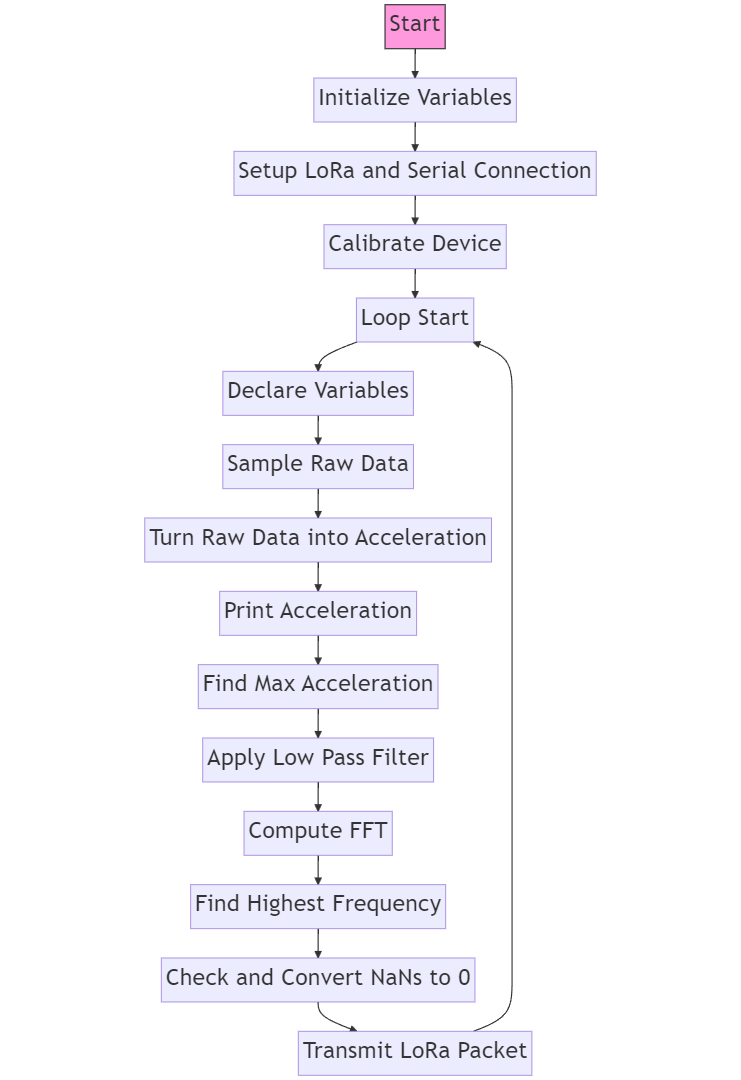
\includegraphics[width=\textwidth]{Sections/Design-Process/proto1-soft-diagram-n.png}
	\label{proto1-soft-diagram}
\end{figure}

\begin{figure}[H]
	\centering 
	\caption{Prototype 1 Software Diagram: Receiver}
	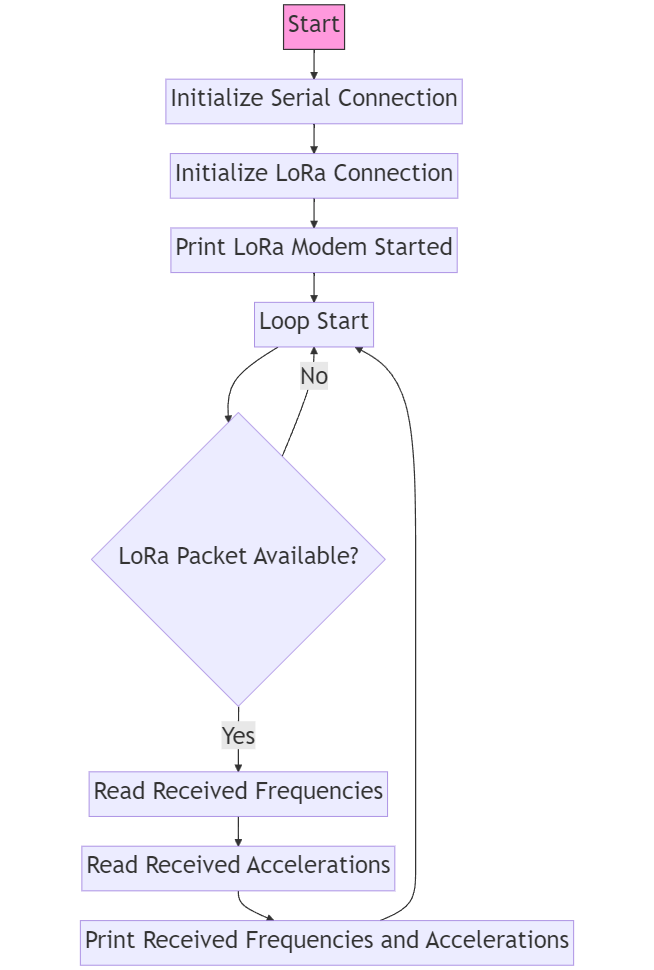
\includegraphics[width=\textwidth]{Sections/Design-Process/proto1-soft-diagram-receiver.png}
	\label{proto1-soft-diagram-receiver}
\end{figure}

\begin{figure}[H]
	\centering 
	\caption{Prototype 1 Software Diagram: Sender \& Receiver Serial Logging}
	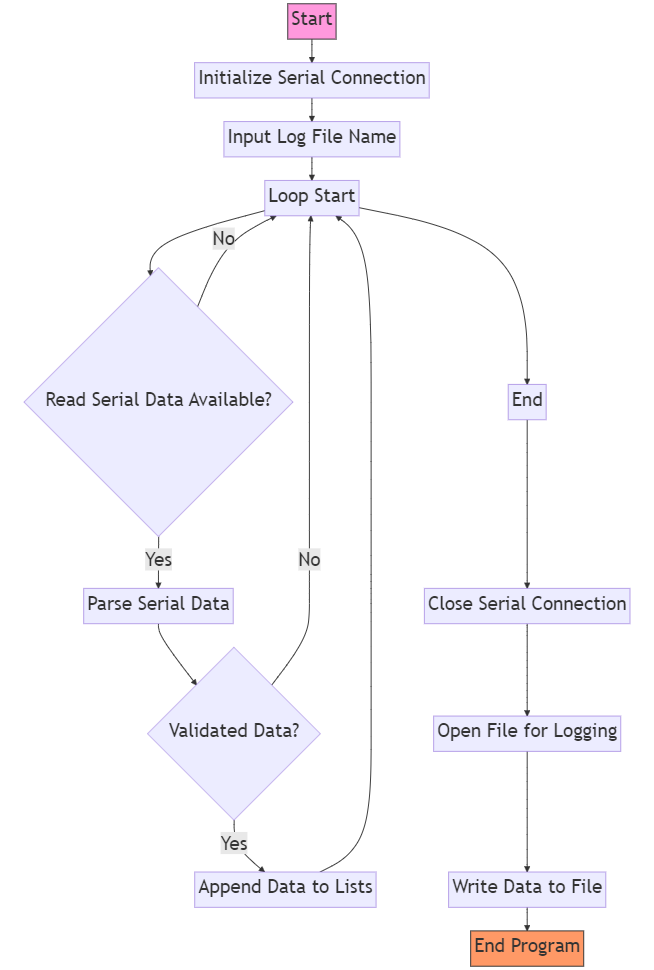
\includegraphics[width=\textwidth]{Sections/Design-Process/proto1-soft-diagram-sender-log.png}
	\label{proto1-soft-diagram-log}
\end{figure}



\begin{figure}[H]
	\centering
	\caption{Prototype 2 Software Diagram}
	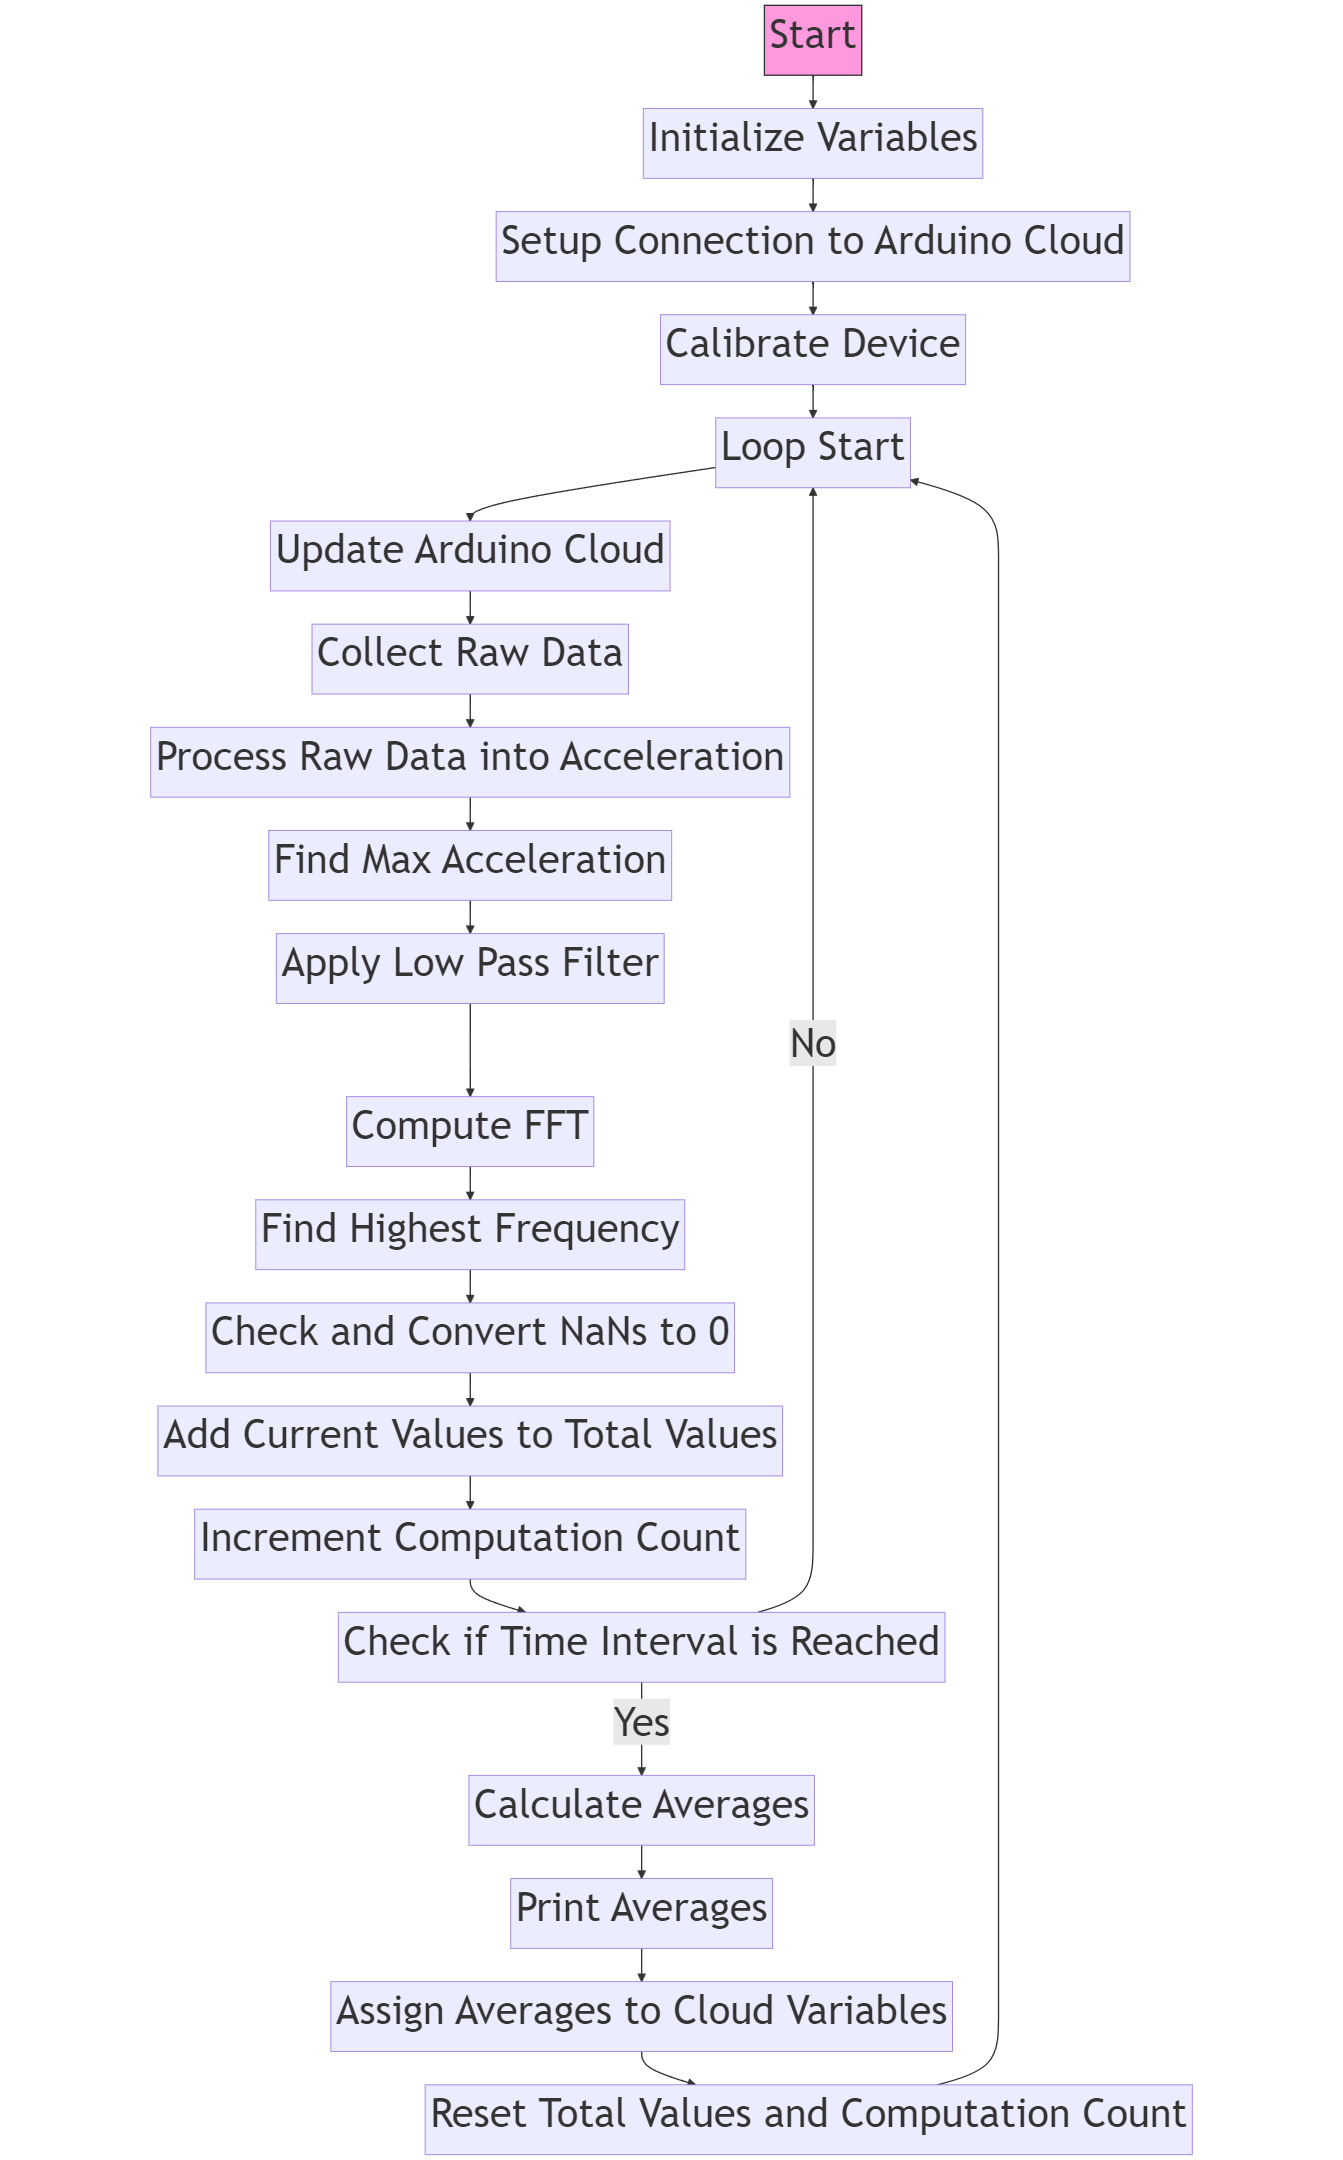
\includegraphics[width=\textwidth]{Sections/Design-Process/proto2-soft-diagram.png}
	\label{proto2-soft-diagram}
\end{figure}

\begin{table}[H]
\begin{tabular}{|ll|}
\hline
\multicolumn{1}{|c|}{\textbf{Step}} & \multicolumn{1}{c|}{\textbf{Process}}                                                                                                          \\ \hline
\multicolumn{2}{|c|}{\textbf{Sender}}                                                                                                                                                \\ \hline
\multicolumn{1}{|l|}{\textbf{1}}    & \begin{tabular}[c]{@{}l@{}}Relevant Arduino and CPP libraries are imported \\ and variables are initialized.\end{tabular}                      \\ \hline
\multicolumn{1}{|l|}{\textbf{2}}    & LoRa and serial connection is initialized.                                                                                                     \\ \hline
\multicolumn{1}{|l|}{\textbf{3}}    & \begin{tabular}[c]{@{}l@{}}The accelerometer is calibrated and zero values are \\ set for each axis.\end{tabular}                              \\ \hline
\multicolumn{1}{|l|}{\textbf{4}}    & The raw acceleration is sampled and processed.                                                                                                 \\ \hline
\multicolumn{1}{|l|}{\textbf{5}}    & The maximum acceleration is found.                                                                                                             \\ \hline
\multicolumn{1}{|l|}{\textbf{6}}    & Low pass filter is applied to the acceleration values.                                                                                         \\ \hline
\multicolumn{1}{|l|}{\textbf{7}}    & FFT is computed and the peak frequency is found.                                                                                               \\ \hline
\multicolumn{1}{|l|}{\textbf{8}}    & NaN values are converted to 0.                                                                                                                 \\ \hline
\multicolumn{1}{|l|}{\textbf{9}}    & \begin{tabular}[c]{@{}l@{}}Max acceleration and frequency values for each\\ axis are converted to bytes and sent via LoRa packet.\end{tabular} \\ \hline
\multicolumn{2}{|c|}{\textbf{Receiver}}                                                                                                                                              \\ \hline
\multicolumn{1}{|l|}{\textbf{10}}   & \begin{tabular}[c]{@{}l@{}}Relevant Arduino and CPP libraries are \\ imported and varaibles are initialized.\end{tabular}                      \\ \hline
\multicolumn{1}{|l|}{\textbf{11}}   & LoRa and serial connection is initialized.                                                                                                     \\ \hline
\multicolumn{1}{|l|}{\textbf{12}}   & \begin{tabular}[c]{@{}l@{}}Check whether there is a LoRa packet to \\ read. The code loops until there is an available packet.\end{tabular}    \\ \hline
\multicolumn{1}{|l|}{\textbf{13}}   & \begin{tabular}[c]{@{}l@{}}When there is an available packet the \\ frequency and acceleration values are decoded and \\ printed.\end{tabular} \\ \hline
\multicolumn{2}{|c|}{\textbf{Logging}}                                                                                                                                               \\ \hline
\multicolumn{1}{|l|}{\textbf{14}}   & \begin{tabular}[c]{@{}l@{}}Relevant Python modules are imported and serial \\ connection is initialized.\end{tabular}                          \\ \hline
\multicolumn{1}{|l|}{\textbf{15}}   & The user enters the name of the log file.                                                                                                      \\ \hline
\multicolumn{1}{|l|}{\textbf{16}}   & \begin{tabular}[c]{@{}l@{}}Check whether there is serial data to read. The code \\ loops until there is available data.\end{tabular}           \\ \hline
\multicolumn{1}{|l|}{\textbf{17}}   & When there is data available it is parsed and validated.                                                                                       \\ \hline
\multicolumn{1}{|l|}{\textbf{18}}   & \begin{tabular}[c]{@{}l@{}}Once validated the data is appended to a list and the \\ serial connection is terminated.\end{tabular}              \\ \hline
\multicolumn{1}{|l|}{\textbf{19}}   & The serial data is written to the specified file.                                                                                              \\ \hline
\multicolumn{2}{|c|}{\textbf{Plotting}}                                                                                                                                              \\ \hline
\multicolumn{1}{|l|}{\textbf{20}}   & Relevant Python modules are imported.                                                                                                          \\ \hline
\multicolumn{1}{|l|}{\textbf{21}}   & The user enters the name of the log file and the plot file.                                                                                    \\ \hline
\multicolumn{1}{|l|}{\textbf{22}}   & The data from the log file is read and plotted.                                                                                                \\ \hline
\multicolumn{1}{|l|}{\textbf{23}}   & \begin{tabular}[c]{@{}l@{}}The plots are saved with the specified file names and \\ displayed to the user.\end{tabular}                        \\ \hline
\end{tabular}
\caption{Prototype 1: Beam Test Software Processing Steps}
\label{proto1-beam-test-soft-steps}
\end{table}

\begin{table}[]
\begin{tabular}{|ll|}
\hline
\multicolumn{1}{|c|}{\textbf{Step}} & \multicolumn{1}{c|}{\textbf{Process}}                                                                                                                                                                \\ \hline
\multicolumn{2}{|c|}{\textbf{Sender}}                                                                                                                                                                                                      \\ \hline
\multicolumn{1}{|l|}{\textbf{1}}    & \begin{tabular}[c]{@{}l@{}}Relevant Arduino and CPP libraries are imported \\ and variables are initialized.\end{tabular}                                                                            \\ \hline
\multicolumn{1}{|l|}{\textbf{2}}    & Connection to Arduino Cloud is established.                                                                                                                                                          \\ \hline
\multicolumn{1}{|l|}{\textbf{3}}    & \begin{tabular}[c]{@{}l@{}}The accelerometer is calibrated and zero values are \\ set for each axis.\end{tabular}                                                                                    \\ \hline
\multicolumn{1}{|l|}{\textbf{4}}    & \begin{tabular}[c]{@{}l@{}}The main loop starts and the Arduino Cloud is \\ updated.\end{tabular}                                                                                                    \\ \hline
\multicolumn{1}{|l|}{\textbf{5}}    & The raw acceleration is sampled and processed.                                                                                                                                                       \\ \hline
\multicolumn{1}{|l|}{\textbf{6}}    & The maximum acceleration is found.                                                                                                                                                                   \\ \hline
\multicolumn{1}{|l|}{\textbf{7}}    & Low pass filter is applied to the acceleration values.                                                                                                                                               \\ \hline
\multicolumn{1}{|l|}{\textbf{8}}    & FFT is computed and the peak frequency is found.                                                                                                                                                     \\ \hline
\multicolumn{1}{|l|}{\textbf{9}}    & NaN values are converted to 0.                                                                                                                                                                       \\ \hline
\multicolumn{1}{|l|}{\textbf{10}}   & \begin{tabular}[c]{@{}l@{}}Current max acceleration and frequency values are \\ added to a running total.\end{tabular}                                                                               \\ \hline
\multicolumn{1}{|l|}{\textbf{11}}   & The loop iteration value is incremented.                                                                                                                                                             \\ \hline
\multicolumn{1}{|l|}{\textbf{12}}   & \begin{tabular}[c]{@{}l@{}}The time passed is checked. If less than timer value \\ the loop resets.\end{tabular}                                                                                     \\ \hline
\multicolumn{1}{|l|}{\textbf{13}}   & \begin{tabular}[c]{@{}l@{}}If the time passed is equal to or greater than the \\ timer value then the averages of the running total \\ values are found using the loop iteration value.\end{tabular} \\ \hline
\multicolumn{1}{|l|}{\textbf{14}}   & \begin{tabular}[c]{@{}l@{}}The average values are printed and assigned to \\ their respective cloud variables.\end{tabular}                                                                          \\ \hline
\multicolumn{1}{|l|}{\textbf{15}}   & \begin{tabular}[c]{@{}l@{}}Total values and loop iteration values are reset and \\ the loop is restarted.\end{tabular}                                                                               \\ \hline
\end{tabular}
\caption{Prototype 2: Bridge Test Software Processing Steps}
\label{proto2-bridge-test-soft-steps}
\end{table}



\begin{table}[h]
\begin{tabular}{|c|c|c|l|}
\hline
\textbf{Library/Module} & \textbf{Prototype} & \textbf{Program}  & \multicolumn{1}{c|}{\textbf{Function}}                                                                                                                           \\ \hline
Arduino                 & 1, 2               & Sender            & \begin{tabular}[c]{@{}l@{}}Provides core Arduino functionality \\ such as reading analog input and \\ serial printing.\end{tabular}                              \\ \hline
Math.h                  & 1, 2               & Sender            & \begin{tabular}[c]{@{}l@{}}Standard C library for mathematical \\ operations such as finding absolute \\ max values and checking for NaN \\ values.\end{tabular} \\ \hline
MKRWAN.h                & 1                  & Sender, Receiver  & \begin{tabular}[c]{@{}l@{}}Standard MKRWAN library for \\ basic LoRa communication and \\ channel masking.\end{tabular}                                          \\ \hline
LoRa.h                  & 1                  & Sender, Receiver  & \begin{tabular}[c]{@{}l@{}}Used to control LoRa \\ communication between devices \\ such as writing to a LoRa packet.\end{tabular}                               \\ \hline
ArduinoFFT.h            & 1, 2               & Sender, Receiver  & \begin{tabular}[c]{@{}l@{}}Used to provide FFT functions such \\ as FFT computing, windowing, DC \\ removal and complex to magnitude \\ conversion.\end{tabular} \\ \hline
serial                  & 1                  & Logging           & \begin{tabular}[c]{@{}l@{}}Used for establishing serial \\ connection to COM devices.\end{tabular}                                                               \\ \hline
matplotlib.pyplot       & 1                  & Plotting          & \begin{tabular}[c]{@{}l@{}}Library used for plotting serial log \\ data.\end{tabular}                                                                            \\ \hline
os                      & 1                  & Logging, Plotting & \begin{tabular}[c]{@{}l@{}}Used for attaching file paths to user \\ specified files.\end{tabular}                                                                \\ \hline
\end{tabular}
\caption{Arduino, CPP \& Python Libraries and Modules}
\label{module-list}
\end{table}



\begin{table}[]
\begin{tabular}{|c|c|c|l|c|}
\hline
\textbf{Parameter}                                                                          & \textbf{Prototype} & \textbf{Program} & \multicolumn{1}{c|}{\textbf{Description}}                                                                                & \textbf{Type}                                                        \\ \hline
\begin{tabular}[c]{@{}c@{}}x\_axis, \\ y\_axis, z\_axis\end{tabular}                        & 1, 2               & Sender           & \begin{tabular}[c]{@{}l@{}}Assign axis values from \\ accelerometer to analog\\  inputs on microcontroller.\end{tabular} & \begin{tabular}[c]{@{}c@{}}static \\ const int\end{tabular}          \\ \hline
adc\_resolution                                                                             & 1, 2               & Sender           & \begin{tabular}[c]{@{}l@{}}Resolution of the \\ microcontroller's 12-bit \\ ADC.\end{tabular}                            & \begin{tabular}[c]{@{}c@{}}static \\ const int\end{tabular}          \\ \hline
vRef                                                                                        & 1, 2               & Sender           & Input voltage for ADC.                                                                                                   & \begin{tabular}[c]{@{}c@{}}const \\ double\end{tabular}              \\ \hline
sensitivity                                                                                 & 1, 2               & Sender           & \begin{tabular}[c]{@{}l@{}}Sensitivity of the \\ accelerometer.\end{tabular}                                             & \begin{tabular}[c]{@{}c@{}}static \\ const \\ double\end{tabular}    \\ \hline
maxFreq                                                                                     & 1, 2               & Sender           & \begin{tabular}[c]{@{}l@{}}Cut-off frequency for \\ acceleration sampling.\end{tabular}                                  & \begin{tabular}[c]{@{}c@{}}static \\ const int\end{tabular}          \\ \hline
sample\_n                                                                                   & 1, 2               & Sender           & \begin{tabular}[c]{@{}l@{}}Set the number of \\ acceleration samples.\end{tabular}                                       & \begin{tabular}[c]{@{}c@{}}static \\ const int\end{tabular}          \\ \hline
sampling\_rate                                                                              & 1, 2               & Sender           & \begin{tabular}[c]{@{}l@{}}Sampling frequency for \\ acceleration sampling.\end{tabular}                                 & \begin{tabular}[c]{@{}c@{}}static \\ constexpr\\ double\end{tabular} \\ \hline
sample\_interval                                                                            & 1, 2               & Sender           & \begin{tabular}[c]{@{}l@{}}Delay for acceleration \\ sampling in milliseconds.\end{tabular}                              & \begin{tabular}[c]{@{}c@{}}static\\ constexpr\\ double\end{tabular}  \\ \hline
LP\_Fc                                                                                      & 1, 2               & Sender           & Low pass cut-off frequency.                                                                                              & \begin{tabular}[c]{@{}c@{}}constexpr\\ double\end{tabular}           \\ \hline
LP\_alpha                                                                                   & 1, 2               & Sender           & \begin{tabular}[c]{@{}l@{}}Low pass filter smoothing \\ factor.\end{tabular}                                             & \begin{tabular}[c]{@{}c@{}}constexpr\\ double\end{tabular}           \\ \hline
window\_type                                                                                & 1, 2               & Sender           & \begin{tabular}[c]{@{}l@{}}Specify window type for \\ FFT.\end{tabular}                                                  & define                                                               \\ \hline
FFT\_dir                                                                                    & 1, 2               & Sender           & Specify FFT direction.                                                                                                   & define                                                               \\ \hline
\begin{tabular}[c]{@{}c@{}}xZero, \\ yZero, zZero\end{tabular}                              & 1, 2               & Sender           & \begin{tabular}[c]{@{}l@{}}Zero values for acceleration\\ calibration.\end{tabular}                                      & double                                                               \\ \hline
\begin{tabular}[c]{@{}c@{}}totalMaxAccelX, \\ totalMaxAccelY,\\ totalMaxAccelZ\end{tabular} & 2                  & Sender           & \begin{tabular}[c]{@{}l@{}}Running total for finding \\ average max acceleration \\ values.\end{tabular}                 & float                                                                \\ \hline
\begin{tabular}[c]{@{}c@{}}totalMaxFreqX, \\ totalMaxFreqY, \\ totalMaxFreqZ\end{tabular}   & 2                  & Sender           & \begin{tabular}[c]{@{}l@{}}Running total for finding \\ average max frequency \\ values.\end{tabular}                    & float                                                                \\ \hline
computationCount                                                                            & 2                  & Sender           & \begin{tabular}[c]{@{}l@{}}Counts the number of loop \\ iterations for finding average \\ max values.\end{tabular}       & int                                                                  \\ \hline
\end{tabular}
\caption{Global Program Parameters}
\label{global-vars}
\end{table}





\subsubsection{Prototype 1 Main Software Loop}
The main software loop for prototype one is displayed in the software diagrams in figure \ref{proto1-soft-diagram}, figure \ref{proto1-soft-diagram-receiver}, figure \ref{proto1-soft-diagram-log}, figure\ref{proto1-soft-diagram-sender-plot} and figure \ref{proto1-soft-diagram-receiver-plot}.\\\\
The sender program is uploaded to the node microcontroller and the receiver program is uploaded to the gateway microcontroller as specified in the system diagram in figure \ref{proto1-sys-diagram}. The reset button on each device is pushed which causes the node microcontroller to calibrate, and the serial and LoRa connections to be established on both devices. The main program on the sender device then starts reading in raw acceleration values from the accelerometer and converts these into m/s/s values. These processed acceleration values are serially printed. The maximum acceleration value for each axis is found and the low-pass filter is applied to the processed acceleration values. FFT objects for each axis are created using the processed acceleration values, number of samples and sampling rate. DC bias is removed by subtracting the mean acceleration from each value and a Hanning window is then applied to the data. The FFT is then computed and the result is converted from complex to magnitude form. The Arduino FFT library's MajorPeak() function is called which returns the peak frequency from the computed FFT. Now, the checkNan() function is called for the maximum acceleration and frequency values to convert any NaN values to zero. A LoRa packet is then created using the LoRa beginPacket() function and the maximum acceleration and frequency values are converted to byte format and written to the packet. The packet is then closed using the LoRa endPacket() function and transmitted to the gateway node.\\\\
The main program on the receiver device checks if a LoRa packet is available to read using the LoRa parsePacket() function. Once there is an available packet the maximum acceleration and frequency values are decoded from bytes to floats and serially printed.\\\\
The logging Python script for the sender and receiver devices are executed and write the serial output from each device to the user specified text file. The logging is ended when the user ends the programming by inputting the control c command.\\\\
The plotting Python script for both devices is then executed and reads the logged data from the user specified text file. The raw acceleration, maximum acceleration and maximum frequency are plotted using Matplotlib's pyplot function and the figures are stored as PNG images with the user specified file name. 

\subsubsection{Arduino Cloud Initialization}
When cloud variables are created on the Arduino IoT Cloud platform, a thingProperties.h header file is automatically generated with the device's app EUI, app key and thing ID. A network mask is applied to the AU915 frequency band to ensure communication over frequency sub band two which is required for the TNN back-end integration. 

\subsubsection{Prototype 2 Main Software Loop}
The main software loop for prototype two is displayed in the software diagram in figure \ref{proto2-soft-diagram}.\\\\
The main code for the sender node in prototype two is similar to that in prototype one with some major key differences, starting with the initialization of the global variables defined in table \ref{global-vars}. The calibration process is identical to prototype one but the setup function now initiates a connection to the Arduino Cloud platform using the device EUI and app key defined in the thingProperties.h header file. At the start of the main loop, the Arduino Cloud update() function is called which updates the initial values of the cloud variables to zero. The raw acceleration is processed in the same way as prototype one, and the maximum acceleration is found, FFT computed and maximum frequency peak is calculated. These maximum values are added to a respective running total value and the computation count is incremented which is used to find the average of these maximum running totals over a 60 second period. Once 60 seconds has passed the averaged maximum values are stored in the cloud variables provided by the thingProperties.h header file. The computation count is then reset to zero. The main loop then calls the update() function again and the updated cloud variables are stored on the Arduino IoT Cloud platform. 

\subsection{Hardware Design}
\subsubsection{PCB Design}
The PCB for this project was designed in Altium Designer. The purpose of this PCB was to replace the breadboard in prototype one with a carrier board for prototype 2, facilitating the connection between the microcontroller, accelerometer and battery pack. A footprint library was initially created to match the dimensions and pin locations of the microcontroller and accelerometer. Each device has a pitch of 2.54mm. The accelerometer footprint can be seen in figure \ref{accel-footprint} and the microcontroller in figure \ref{micro-footprint}. The pink mesh represents the mechanical keep-out layer which matches the physical dimensions of each device. The physical dimensions of the accelerometer were width 15mm and length 18mm. The physical dimensions of the microcontroller were width 25mm and length 67.6mm. 

\begin{figure}[H]
	\centering 
	\caption{Accelerometer PCB Footprint}
	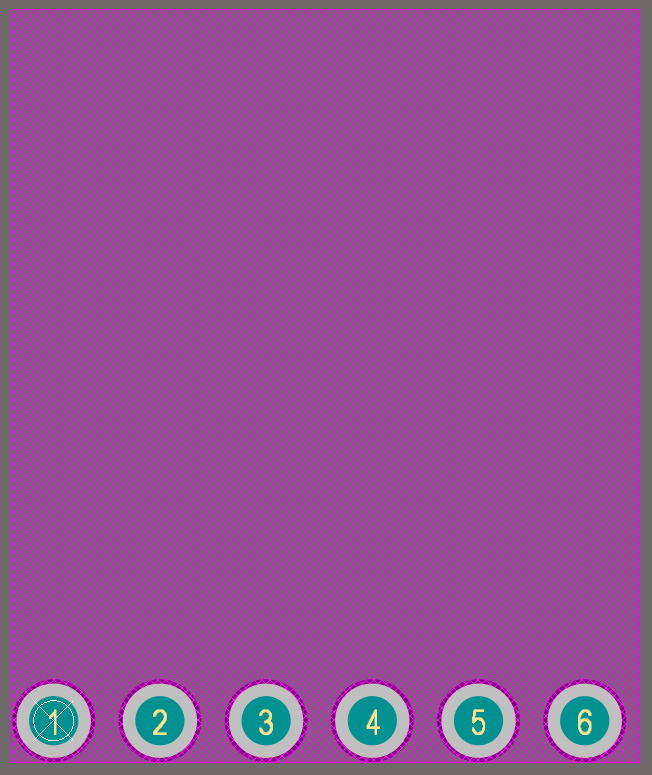
\includegraphics[width=.4\textwidth]{Sections/Design-Process/accel-footprint.png}
	\label{accel-footprint}
\end{figure}

\begin{figure}[H]
	\centering
	\caption{MKRWAN1300 PCB Footprint}
	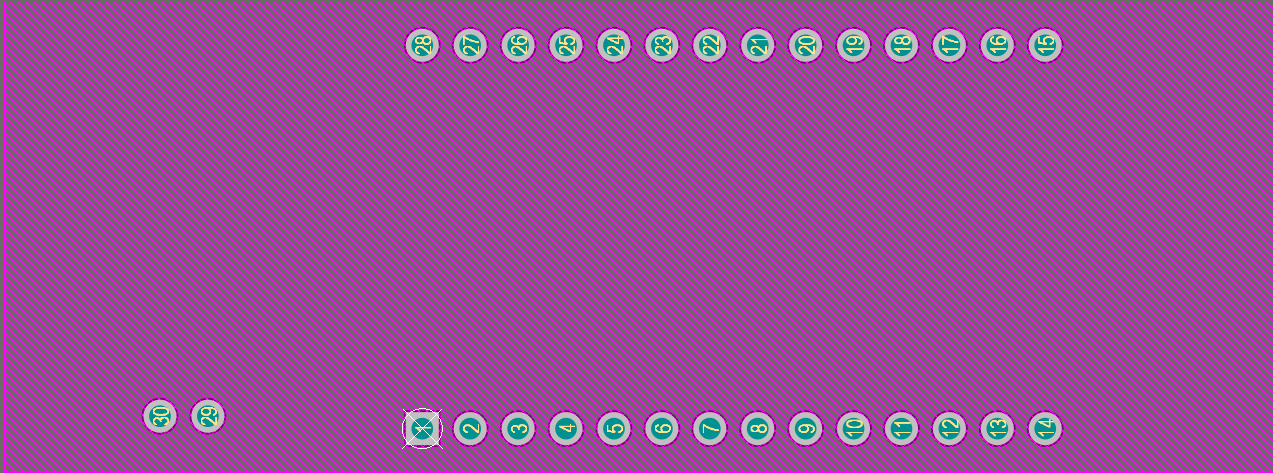
\includegraphics[width=.6\textwidth]{Sections/Design-Process/micro-footprint.png}
	\label{micro-footprint}
\end{figure}

\clearpage

A schematic library was then created with symbols for each device. These symbols contain nets for each of the pins on both devices. The symbol for the accelerometer is shown in figure \ref{accel-symbol} and the microcontroller in figure \ref{micro-symbol}. 

\begin{figure}[H]
	\centering
	\caption{Accelerometer SCH Symbol}
	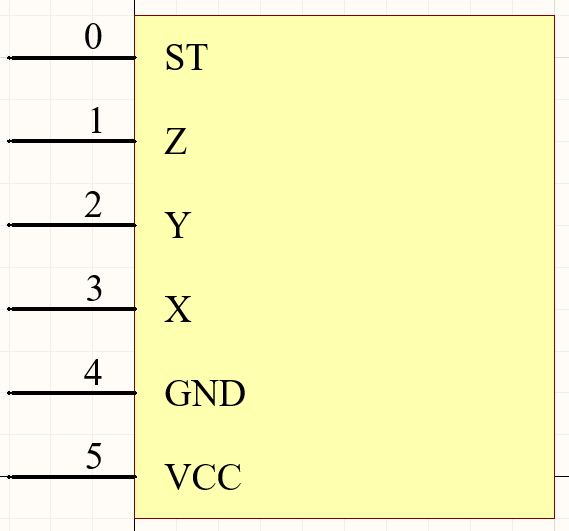
\includegraphics[width=.4\textwidth]{Sections/Design-Process/accel-symbol.png}
	\label{accel-symbol}
\end{figure}

\begin{figure}[H]
	\centering
	\caption{MKRWAN1300 SCH Symbol}	
	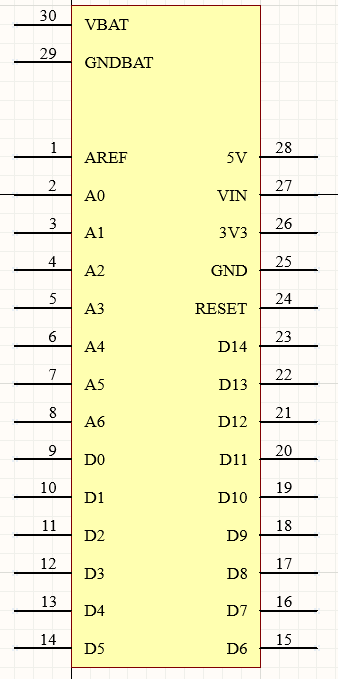
\includegraphics[width=.3\textwidth]{Sections/Design-Process/micro-symbol.png}
	\label{micro-symbol}
\end{figure}

The symbols are used to create the schematic of the PCB, and the correct connections between the accelerometer and microcontroller pins are traced. The full schematic can be seen in figure \ref{PCB-schematic}. The schematic was then imported into a PCB document and the board was created with width 147.6mm, height 31mm and a thickness of 0.4mm. The trace width was set to 0.254mm and tear drops were added to each pin connection. Mounting holes with 2mm diameter were added to each corner of the PCB for enclosure mounting, and labels for the microcontroller and accelerometer were added to the top overlay. The 2D layout is shown in figure \ref{PCB-2D} and the 3D layout is shown in figure \ref{PCB-3D}.

\begin{figure}[H]
	\centering
	\caption{PCB Schematic}	
	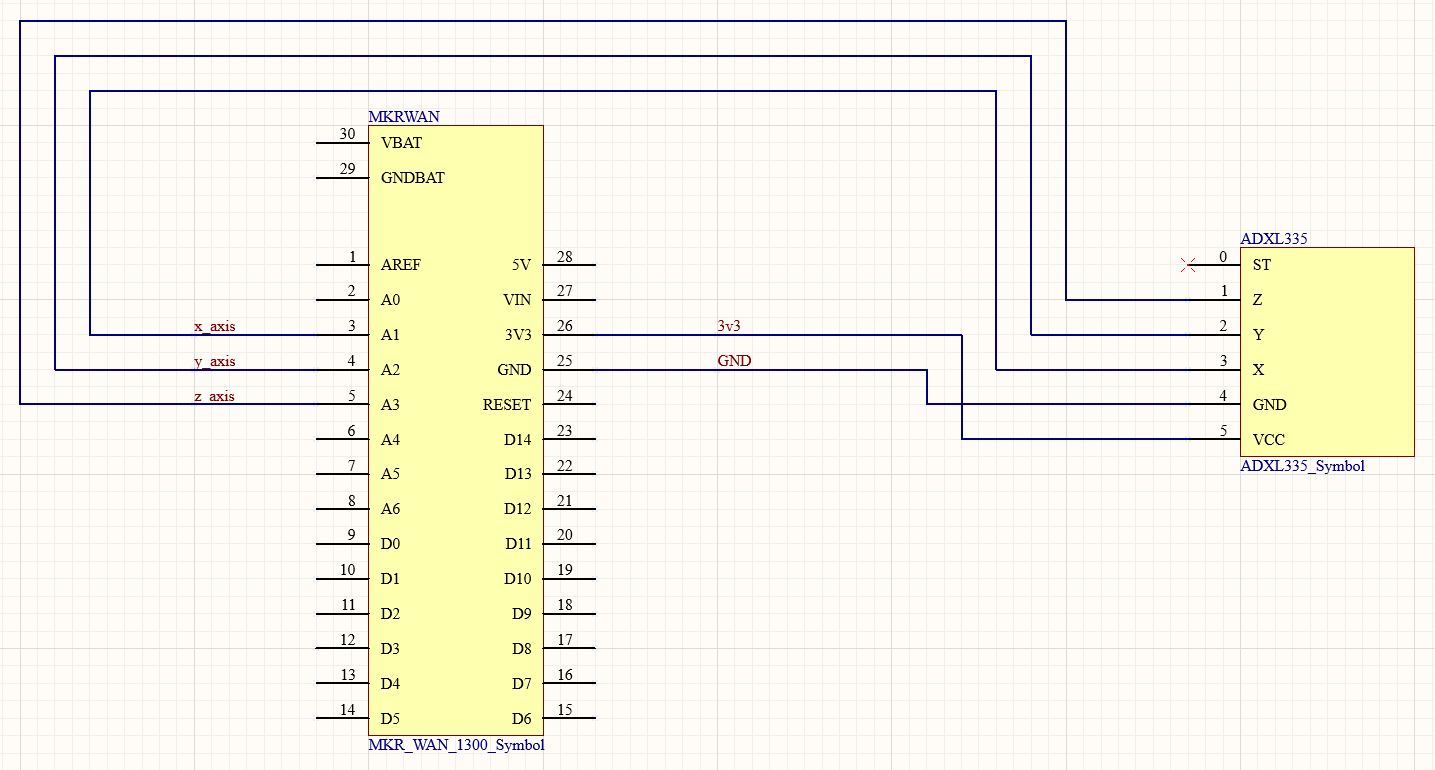
\includegraphics[width=\textwidth]{Sections/Design-Process/PCB-schematic.png}
	\label{PCB-schematic}
\end{figure}

\begin{figure}[H]
	\centering
	\caption{PCB 2D Layout}	
	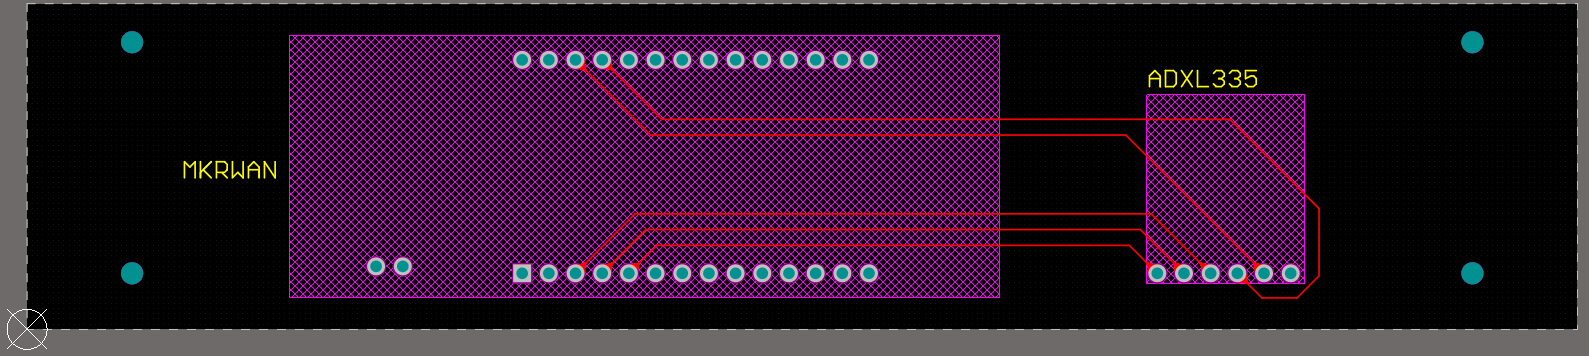
\includegraphics[width=\textwidth]{Sections/Design-Process/PCB-2D.png}
	\label{PCB-2D}
\end{figure}

\begin{figure}[H]
	\centering
	\caption{PCB 3D Layout}	
	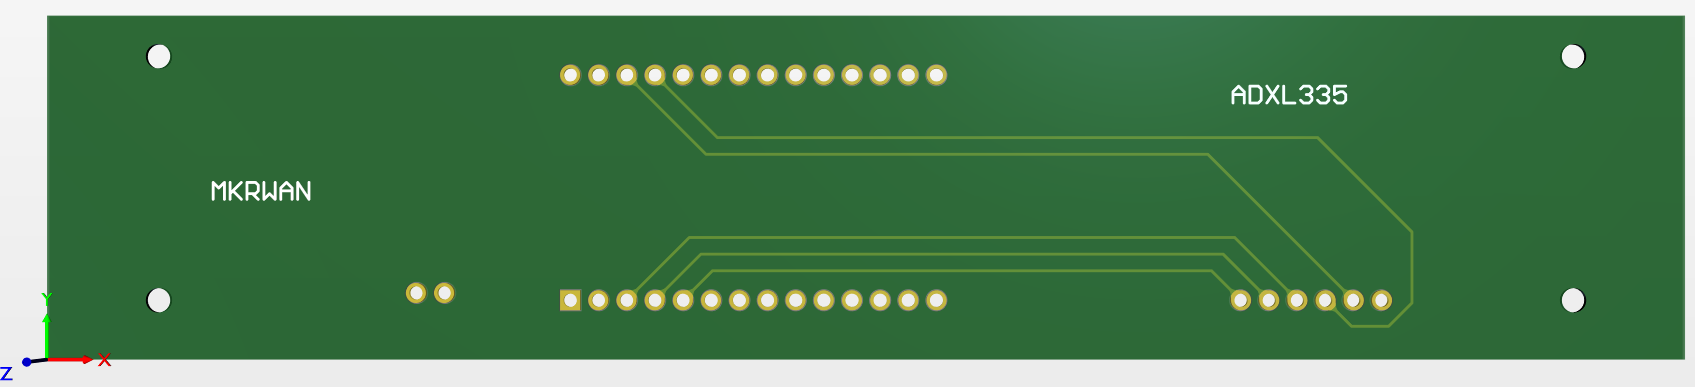
\includegraphics[width=\textwidth]{Sections/Design-Process/PCB-3D.png}
	\label{PCB-3D}
\end{figure}

\clearpage

\subsubsection{Enclosure Design}
The enclosure for this project was designed in OnShape CAD software. The enclosure was designed to sit perfectly behind the handrail of the Griffith footbridge. The enclosure was 3D printed at Griffith University using hard PETG filament. In order to fit the enclosure onto the 3D printer it had to be designed with a front and back plate which was secured together using six M3 heat set-ins and six M3 20mm machine screws. The lid for this enclosure was designed with an overlap and was secured to the top of the enclosure using four of the same M3 heat set-ins and four M3 20mm machine screws. In order to install the heat set ins, the enclosure was printed with holes of 4mm and the heat set-ins were melted into these holes using a soldering iron. Four M2 30mm screws were used to secure PCB mounts to the back plate of the enclosure, and the PCB was fastened to these mounts using four M2 nuts. The enclosure was printed with a pass-through hole for an M10 bolt that was used to secure the enclosure to the bridge and an M10 nut was used to fasten the bolt to the enclosure. A shelf was created on the right side of the enclosure for the battery pack to sit within. An exploded view of this enclosure can be seen in figure \ref{enclosure-explode} and the bridge installation can be seen in figure \ref{enclosure-wall}. The inside of the enclosure is displayed in figure \ref{enclosure-inside} and the installation on the Griffith footbridge can be seen in figure \ref{enclosure-griffith}. 

\begin{figure}[H]
	\centering
	\caption{Enclosure Explode View}	
	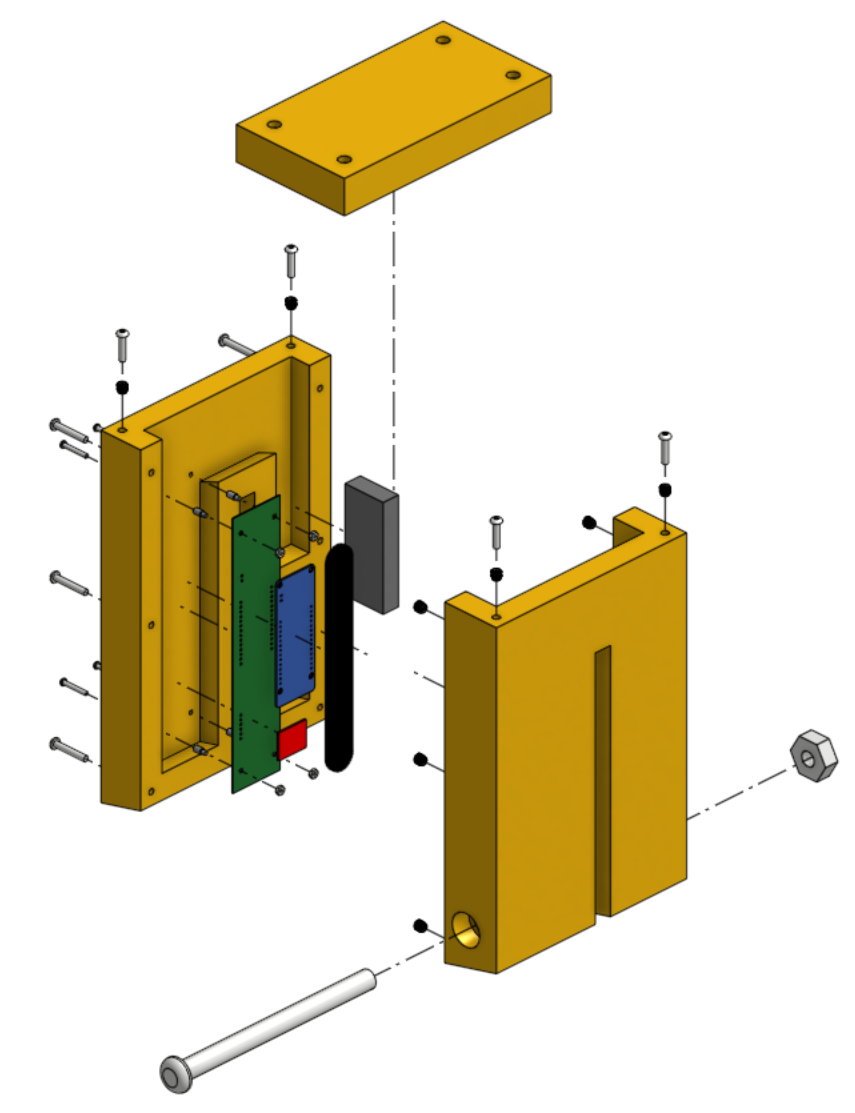
\includegraphics[scale=0.42]{Sections/Design-Process/enclosure-explode.png}
	\label{enclosure-explode}
\end{figure}
\clearpage 
\begin{figure}[H]
	\centering
	\caption{Enclosure Bridge Installation}	
	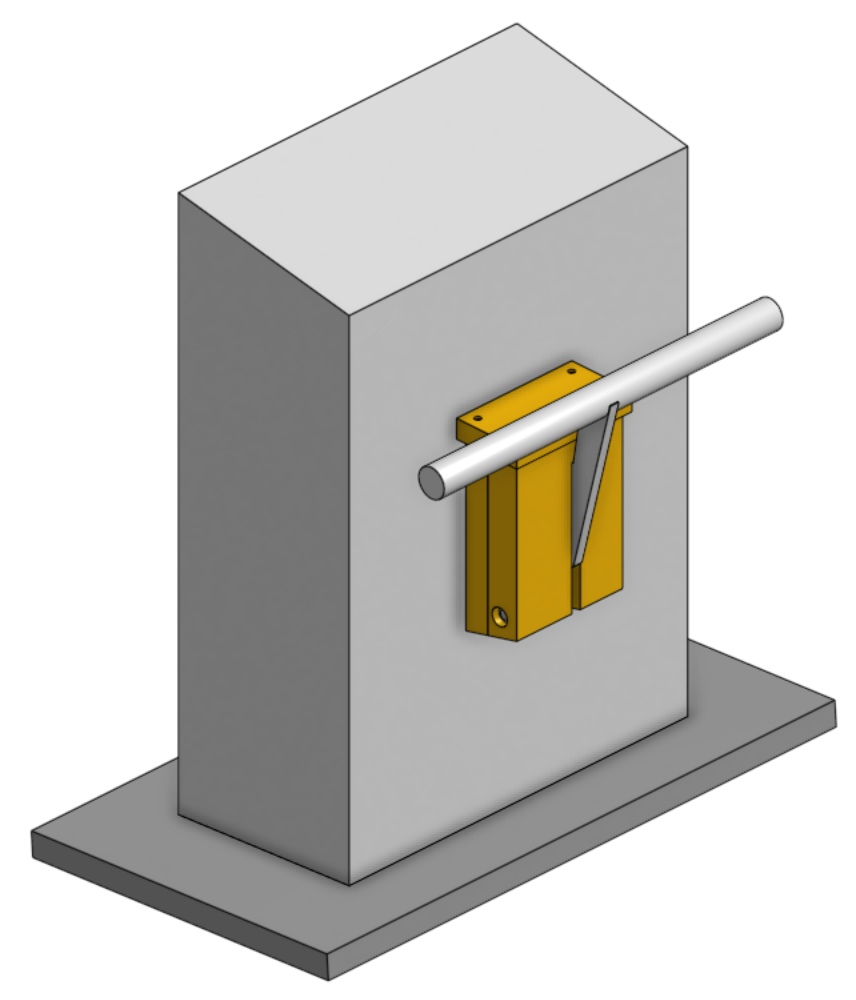
\includegraphics[scale=0.45]{Sections/Design-Process/enclosure-wall.png}
	\label{enclosure-wall}
\end{figure}

\begin{figure}[H]
	\centering
	\begin{subfigure}{.5\textwidth}
		\centering 
		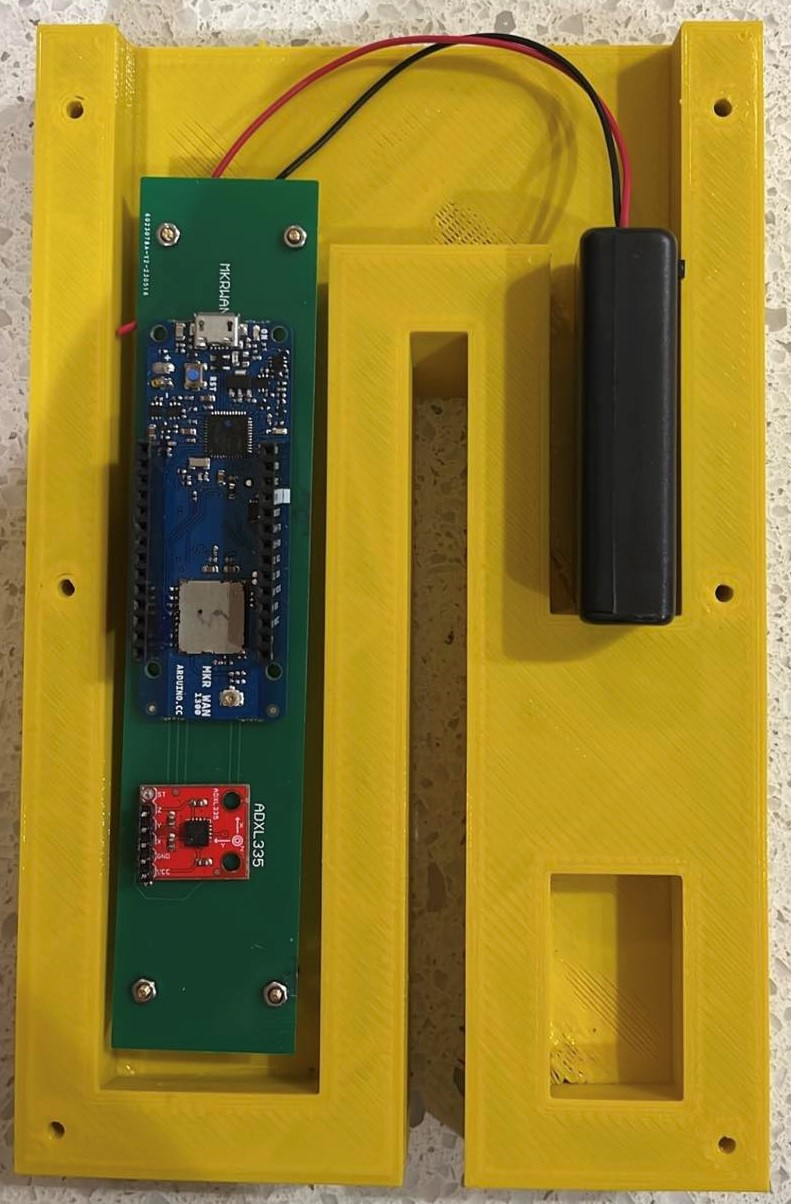
\includegraphics[scale=0.3]{Sections/Design-Process/enclosure-inside.jpg}
		\caption{Inside of Enclosure}
		\label{enclosure-inside}
	\end{subfigure}%
	\begin{subfigure}{.5\textwidth}
		\centering
		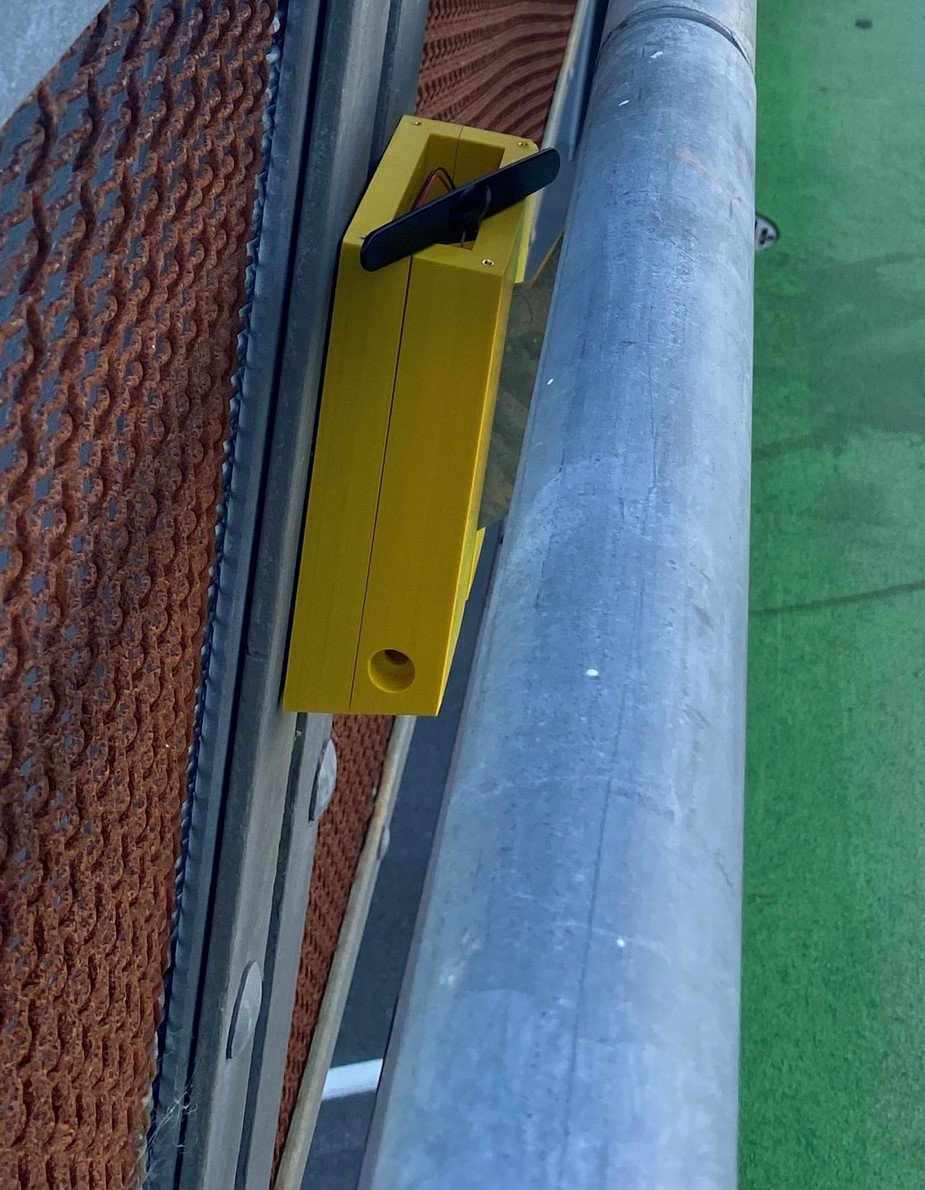
\includegraphics[scale=0.3]{Sections/Design-Process/enclosure-griffith.png}
		\caption{Enclosure Griffith Footbridge Installation}
		\label{enclosure-griffith}
	\end{subfigure}
	\caption{Enclosure Integration}
	\label{enclosure-integration}
\end{figure}

\subsection{Packet Transmission}
Data transmission calculations were conducted using the TNN's LoRaWAN airtime calculator \cite{airtime-calc}. According to Australian communication laws, LoRa packets must be transmitted on the AU915 frequency band between 915-928MHz. As part of this restriction, messages must adhere to a 1\% duty cycle. Since the message payload contains six float values, the payload itself is 24 bytes in size. Adding the overhead of 12 bytes, which contains information such as the device address and frame counter, the total packet size is 36 bytes. The Arduino IoT Cloud platform uses Adaptative Data Rate (ADR) to automatically determine the most suitable spreading factor (SF) for transmission. For the case of this project, a spreading factor of 7 is suitable for a connection up to 2km. The SF7BW125 data rate needs a minimum of 77.06ms airtime to transmit a message size of 36 bytes. Accounting for the 1\% duty cycle this gives a minimum requirement of 7.71 seconds between subsequent messages on the same sub band allowing for a total of 467 messages to be sent per hour. Adhering to the restrictions of the TNN fair access policy, the data rate is restricted to 30 seconds of air time per device per day, which imposes a limit of 389 messages per day with a 36 byte packet size. Finally, if the device is transmitting all day, a maximum of 16.2 message per hour can be sent. 









